\documentclass{beamer}

\usepackage[english]{babel}
\usepackage[utf8x]{inputenc} 	
\usepackage{caption}
\usepackage{adjustbox}
\usepackage{amsmath}


%\documentclass[tikz,border=10pt]{standalone}


%% graph drawing
\usepackage{tikz}
\usetikzlibrary{positioning}
\usetikzlibrary{overlay-beamer-styles}
\tikzset{block/.style={rectangle, draw, text width=6em, text centered, rounded corners, minimum height=3em}}



% Title format
\title{Fragment Assembly in succint space}
\subtitle{Compressing de Bruijn and Overlap graphs}
\titlegraphic{
\includegraphics[height=1.5cm, width=1.5cm]{img/cherubino_unipi.eps}}
\author{Lapo Toloni}
\institute{Seminar for the course Bioinformatics.\\ MsC in Computer Science, Università di Pisa, a.a. 2018/2019}
\date{2nd, August 2019}

% Theme definition
\usetheme{Berlin} 
\useinnertheme{rounded}
\useoutertheme{miniframes} 
\setbeamercovered{dynamic}

% Set theorem style
\theoremstyle{definition}
\newtheorem{claim}{Claim:}
%%%%%%%%%%%%%%%%%%%%
%% Starting point %%
%%%%%%%%%%%%%%%%%%%%
\begin{document}
	
% First slide: Frontmatter
\begin{frame}
\maketitle
\end{frame}


% BLUE-BLOCK \begin{block}{titolo}\end{block} 
% GREEN-BLOCK exampleblock
% RED-BLOCK alertblock

%%%%%%%%%%%%%%%%%%%%%%%%%%%%%%%%%%%%%%%%%%%%%%%%%%%%%%%%%%%%%%%%%%%%%%%%%%%%%%%%
%%%%%%%%%%%%%%%%%%%% INCLUDE SECTIONS PART %%%%%%%%%%%%%%%%%%%%%%%%%%%%%%%%%%%%%
%%%%%%%%%%%%%%%%%%%%%%%%%%%%%%%%%%%%%%%%%%%%%%%%%%%%%%%%%%%%%%%%%%%%%%%%%%%%%%%%
%%%%%%%%%%%%%%%%%%%%%%%%%%%%%%%%%%%%%%%%%%%%%%%%%%%%%%%%%%%%%%%%%%%%%%%%%%%%%%%%
% Section 1
\section{Genome Assembly Problem}

\begin{frame}
\frametitle{DNA Assembly}
Within the last two decades, \textbf{assembling a genome from an enormous amount of reads} from various DNA sequencers has been one of the most challenging computational problems in molecular biology.
\\ \medskip
Such a problem is proved to be NP-hard and many algorithms have been devised to come to a solution both exact and approximated.
\\ \medskip
There are two types of algorithms that are commonly utilized by assemblers:
\begin{itemize}
\item \textbf{Greedy}, which aim for local optima,
\item \textbf{Graph methods}, which aim for global optima.
\end{itemize}
\end{frame}

\begin{frame}
\frametitle{Graph methods (Waterman and Gene Myers 1994)}
Graph-method-assemblers come in two varieties: the ones based on \textbf{overlap graph} and the others based on \textbf{de Bruijn graphs}.
\\ \medskip 
These methods represented an important step forward in sequence assembly, as they both use algorithms to reach a global optimum instead of a local one.
Thanks to these theoretical advances computational genomics over large volumes of data became an easier problem to attack.
\\ \medskip
Both of these methods made progress towards better assemblies  but nowadays the De Bruijn graph method has become the most popular due to the so called \textcolor{red}{next-generation sequencing machines}.
\end{frame}

\begin{frame}
\frametitle{The Overlap graph}
Most assembly algorithms from the \textit{"Sanger era"}
are based on the \textbf{overlap graph}.
\\ \medskip
Such a graph has one node for each read produced by the sequencing process and two nodes are connected by a weighted edge iff the corresponding two reads have an overlap of enough length. \textit{(this length is a parameter of the implementation)}
\begin{figure}
	Read set $\mathcal{R} = \{CTCTAGGCC, GCCCTCAAT, CAATTTTT\}$
	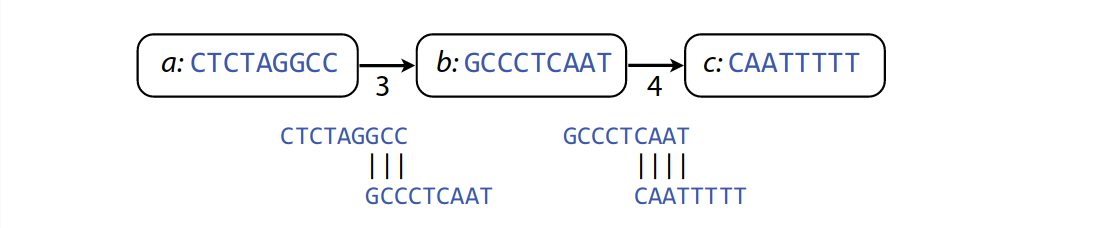
\includegraphics[scale=0.33]{img/overlap-graph-simple.png}
\end{figure}
\end{frame}


\begin{frame}
\frametitle{Shortest common superstring and TSP}
\begin{columns}
	\column{0.5\textwidth}
	By adding a minus sign in front of each edge label we get into a framework
	such that the assembly problem is reduced to the \textbf{Shortest common superstring problem} that indeed is equivalent to \textbf{TSP}, one of the most famous NP-HARD problems.
	\column{0.5\textwidth}
	\begin{figure}
		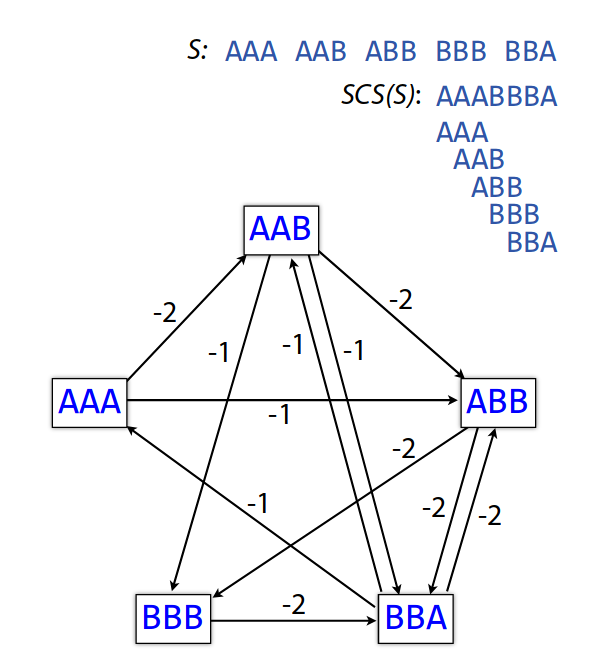
\includegraphics[scale=0.25]{img/tsp-scs.png}
	\end{figure}
\end{columns}
\end{frame}

\begin{frame}
\frametitle{New Generation Sequencing}
This strategy is too expensive to apply against the huge data from most recent \textbf{next-generation sequencers } (NGSs). 
\\ \medskip
NGS machines can sequence vast amount of genome data. 
\\
It makes it computationally not tractable to compare all the pairs of reads to find the optimal solution for \textbf{SCS}. 
\\ \medskip
Moreover, most NGSs cannot read long DNA fragments (e.g., at most 200bp in the case of Illumina HiSeq2000),
and their read lengths are not long enough to detect overlaps with enough lengths between reads.
\end{frame}

\begin{frame}
\frametitle{New Generation Sequencing - Shotgun sequencing}
\begin{columns}
	\column{0.45\textwidth}
	One current popular NGS method is \textbf{shotgun sequencing}, which:
	\begin{itemize}
		\item  clones the genome a bunch of times,
		\item  then randomly breaks each clone into short segments
	\end{itemize}
	the fact that we randomly cut many clones of the same DNA segment should lead to have overlapping reads.
	\column{0.55\textwidth}
	\begin{figure}
		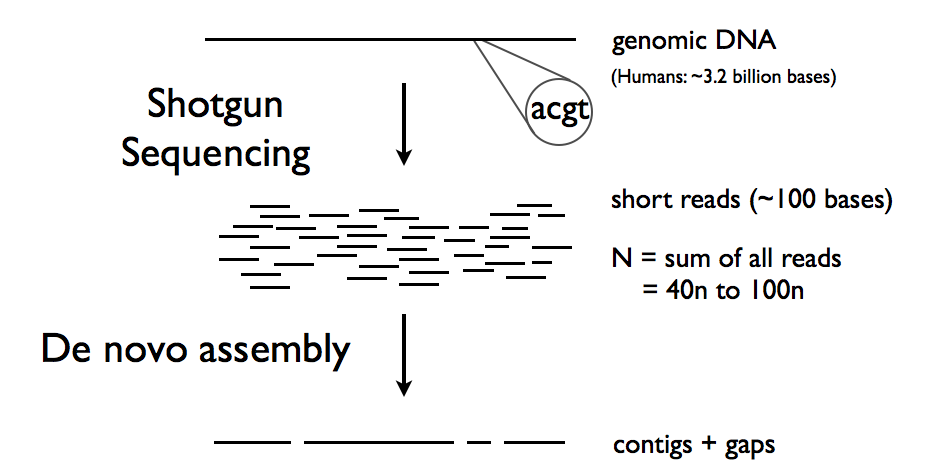
\includegraphics[scale=0.2]{img/shotgun.png}
	\end{figure}
\end{columns}
\end{frame}

\begin{frame}
\frametitle{de Bruijn graph}
\begin{columns}
	\column{0.6\textwidth}
To conquer these problems, many recent assembler algorithms utilize a
graph called the de Bruijn graph.
\\ \medskip
This kind of graphs is really suitable to represent a large network of overlapping \textbf{short read data}.
\\ \medskip
In this model each node represents a \textbf{k-mer} that exists in the reads, and an edge exists iff there is an exact
overlap of length \textbf{k−1} between the corresponding k-mers.
	\column{0.4\textwidth}
	\begin{figure}
	Example read $R =TACGACGTCGACT$
	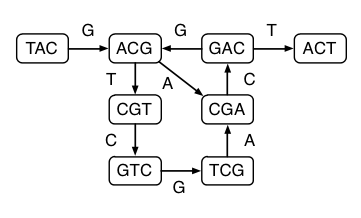
\includegraphics[scale=0.4]{img/dbg-graph-simple.png}
	\end{figure}
\end{columns}
\end{frame}

%\begin{frame}
%\frametitle{de Bruijn graph in Bioinformatics}
%During the assembly of the De Bruijn graph, reads are broken into smaller fragments of a specified size, k.
%\\ \medskip
%The k-mers are then used as nodes in the graph assembly.\\
%Nodes that overlap by some amount (generally, k-1) are connected by a labelled edge.
%\\ \medskip
%The assembler will construct sequences based on the De Bruijn graph. 
%\end{frame}

\begin{frame}
\frametitle{Eulerian path in de Bruijn graphs}
After having built such a graph our original problem reduced to find \textbf{Eulerian paths} in it
\\ \medskip
Assuming \textbf{perfect sequencing} where each length-k substring is sequenced exactly once with no errors,\\
the naive "sliding-window" procedure to build the dBG always yields an Eulerian graph.
\end{frame}

\begin{frame}
\frametitle{dBG PRO and CONS}
The Single most important benefit of De Bruijn graph assemblers is speed and simplicity.
\\ \medskip
But since reads are immediately split into shorter k-mers
\begin{itemize}
	\item Information about contexts longer than k is lost
	\item Read coherence is lost: some paths through De Bruijn graph are inconsistent with respect to input reads. \\
	\item dBGs need to be preprocessed because of an high probability of sequening errors (tips, bubbles ...)
\end{itemize}
\end{frame}

\begin{frame}
\frametitle{Real world cases need something smaller and faster!}
de Bruijn graphs can be constructed more efficiently than the overlap graph in many cases, but naive procedures still remain a bottleneck in term of used space.
\\ \medskip
This is because storing all the edges of the de Bruijn graph requires huge amount of memory.
\\ \medskip 
Thus the focus of this presentation is on reducing the memory required for the de Bruijn graphs deploying some smart compression technique.
\end{frame} % intro to assembly problem
%%%%%%%%%%%%%%%%%%%%%%%%%%%%%%%%%%%%%%%%%%%%%%%%%%%%%%%%%%%%%%%%%%%%%%%%%%%%%%%%
% Section 2
\section{Succint Data Structures}

\begin{frame}
\frametitle{Succint data structures}
A succint space data structure 
\begin{itemize}
	\item stores combinatorial objects using space asymptotical equal to the information theoretic lower bound.
	\item supports operations on its elements in $\mathcal{O}$(1) time.
\end{itemize}
\medskip
Note that if the input is taken from a set of $\mathcal{L}$ distinct combinatorial objects then its information-theoretic lower bound is $\lceil log\ \mathcal{L}\rceil $ bits.
\end{frame}

\begin{frame}
\frametitle{Simple lower bounds}
\underline{Example 1}: \textbf{n elements sets} $\mathcal{S} \subseteq \{1, 2, .., n\}$:
\[ log\ 2^n = n\ bits \]

\medskip

\underline{Example 2}: \textbf{length-n strings}:
\[ n\ log\ \sigma\ bits\ (where\ \sigma\ is\ the\ alphabet\ size) \]

\underline{Example 3}: \textbf{n nodes ordered trees}
\[ log\ \frac{1}{2n-1} \binom{2n-1}{n-1} = 2n - \Theta(log\ n) \]
\end{frame}


\begin{frame}
\frametitle{Some insights}
For any data kind there exists a succint representation 
\begin{itemize}
	\item simply obtained by enumerating and assign codes to every possible objects.
	\item that can be represented in $\lceil log\ \mathcal{L} \rceil$ bits
\end{itemize}
Unluckily not every representation is fine.\\
We need compressed structures upon we can implement fast operations.
\end{frame}

\begin{frame}
\frametitle{Rank / Select queries}
Rank and select are the bread and butter of succinct data structures.
\\
Infact almost every operation on these structures can be implemented combining rank and select queries.
\medskip
\begin{itemize}
\item $\mathbf{rank_c(i)}$   = \#occurences of \textbf{c} in the range [0,i]
\item $\mathbf{select_c(i)}$ = position of the i-th occurrence of \textbf{c}. 
\end{itemize}
\begin{figure}
	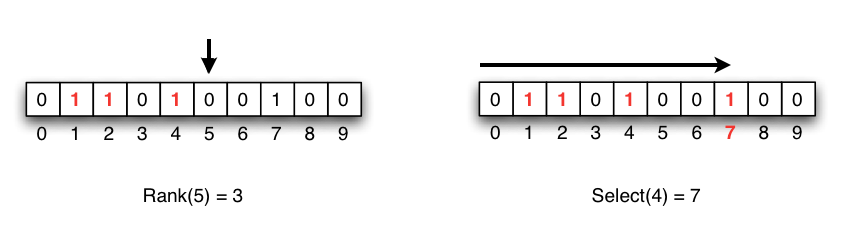
\includegraphics[scale=0.33]{img/ranksel.png}
\end{figure}
\end{frame}


\begin{frame}
\frametitle{Rank / Select queries - Continued}
Speaking of patterns of use, it may also help to keep in mind:
\begin{itemize}
	\item rank is for \textbf{counting}; \\
	two rank queries can count over a range.
	\item select is for \textbf{searching}; \\
	two select queries can find a range
\end{itemize}
\begin{figure}
	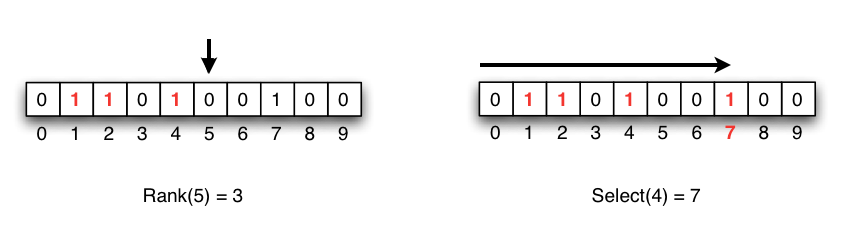
\includegraphics[scale=0.33]{img/ranksel.png}
\end{figure}
\end{frame}


\begin{frame}
\frametitle{Rank / Select queries - Performances}
\begin{itemize}
	\item Assuming that our alphabet size is $ \sigma = polylog(N)$
	ranks and selects can both be done in $\mathcal{O}$(1) time
	by building over our bitvectors simple \textbf{RRR} structures. These additional structures requires just logarithmic space!
	\item for larger alphabets we could use wavelet trees achieving $\mathcal{O}(log \ \sigma)$. Even in this case by using huffman-shaped wavelet trees we can achieve sublinear space usage.
\end{itemize} 
\end{frame}
 % intro to succint data structures
% Section 3
% BOSS and voBOSS
\section{BOSS}

\begin{frame}
\frametitle{Succint de Bruijn Graphs - (Bowe, Sadakane, 2012)}
\textcolor{red}{Achievement}: $4+o$(1) bits per edge (independent of k)
\\ \medskip
Inspiration taken from:
\begin{itemize}
	\item BW Transform [Burrows, Wheeler 94]	
	\item XBW Transform [Ferragina et al. 05]
\end{itemize}
\end{frame}

\begin{frame}
\frametitle{Succint de Bruijn Graphs - Three arrays to represent a graph}
Assuming that \textbf{m} is the number of edges of the graph
\begin{enumerate}
	\item take each k-mer and \textbf{sort} them in reverse lexicographical order
	\\ $\Rightarrow$ Array \textbf{Node} - \textcolor{red}{Don't worry we won't store it explicitly}.
	\item store for each node the label of its outgoing edges 
	\\ $\Rightarrow$ Array \textbf{W}
	\item store a bitvector \textbf{L} of size \textbf{m} whose entries are: $L[i] = 1 \Leftrightarrow Node[i] ≠ Node[i+1]$ \\
	i.e.: indicates the range in which Node refers the same node
	\\ $\Rightarrow$ Array \textbf{L}
\end{enumerate}
\end{frame}

\begin{frame}
\frametitle{Succint de Bruijn Graphs - visualising BOSS}
\begin{columns}
	\column{0.5\textwidth}
	\begin{figure}
		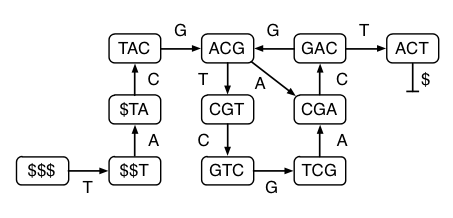
\includegraphics[scale=0.4]{img/sdbg-graph-padded.png}
	\end{figure}
	\column{0.5\textwidth}
	\begin{figure}
		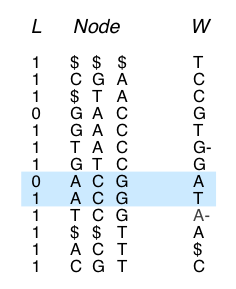
\includegraphics[scale=0.5]{img/sdbg-arrays-1.png}
	\end{figure}
\end{columns}
\end{frame}

\begin{frame}
\frametitle{Optimizing space}
\begin{columns}
	\column{0.5\textwidth}
	Instead of storing the node labels we can save space by just storing the final column of the node labels.
	\\ \medskip
	Since the node labels are sorted, it is equivalent to store an array of first positions. \\ \medskip
	Array \textbf{Node} $\Rightarrow$ Array \textbf{F}
	\column{0.6\textwidth}
	\begin{figure}
		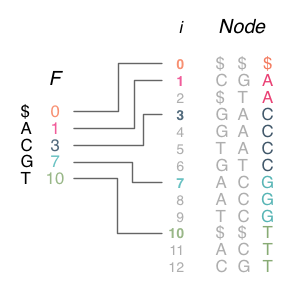
\includegraphics[scale=0.5]{img/f-array.png}
	\end{figure}
\end{columns}
\end{frame}

\begin{frame}
\frametitle{Total space used}
Assuming that our graph has \textbf{m} edges we get:
\begin{enumerate}
	\item Array \textbf{L} $\Rightarrow$ $m$ bits
	\item Array \textbf{W} $\Rightarrow$ $m\ log\ 2^\sigma\ =\ 3\ m$ (in case of DNA alphabet)
	\item Array \textbf{F} $\Rightarrow$ $\sigma\ log\ m\ =\ o(m)$
\end{enumerate}
So total space required is  $4+o$(1) bits per edge. 
\end{frame}



\begin{frame}
\frametitle{Fast travelling across the succint dBG}
Recall that \textbf{DNA sequences can be reconstructed by moving between nodes of the dBG graph}.
\\ \medskip
So we need some way, \textcolor{red}{hopefully fast}, to move through nodes and edges.
\\ \medskip
Thanks to two simple observations derived from how we succintly represented our graph and rank / select queries support for two of our three vectors we will achieve the wished speed of use.
\end{frame}

\begin{frame}
\frametitle{BOSS properties - 1}
\begin{claim}[1]
	All the edges going out from a node are next each other in the representation
\end{claim}
\begin{figure}
	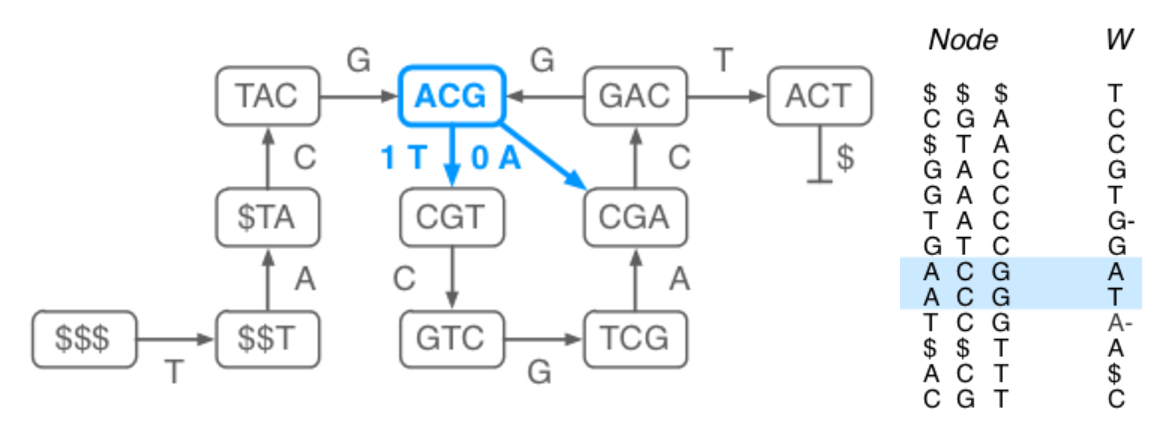
\includegraphics[scale=0.25]{img/claim1.png}
\end{figure}
\end{frame}

\begin{frame}
\frametitle{BOSS properties - 2}
\begin{claim}[2]
	Nodes labels in the last column of \textbf{Node} maintain the same relative order as the edge labels in \textbf{W}.
\end{claim}
\begin{figure}
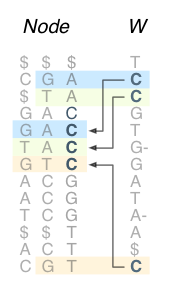
\includegraphics[scale=0.45]{img/claim2.png}
\end{figure}
\end{frame}

\begin{frame}
\frametitle{Some other observations}
\begin{enumerate}
	\item In a dBG every node is defined by its previous k edges.
	\item It may be the case that we need to disambiguate between edges that exit separate nodes but have the same label and enter the same node. (flagged labels in \textbf{W})
	\item Since a 1 in the \textbf{L} vector identifies a unique node,\\ 
	we can use this vector to index nodes (\textbf{HINT}: use $select_1$),\\
	whereas standard array accesses refer to edges.
\end{enumerate}
\end{frame}

\begin{frame}
\frametitle{Basic navigation: going forward and backward}
In order to support some public interface to navigate the graph, we first devise two simple procedures based on rank and select queries to work with edges: 
\begin{itemize}
	\item \textbf{forward(i)}: returns the index of the last edge of the node pointed by edge i.
	\item \textbf{backward(i)}: returns the index of the first edge that points to the node that the edge at i exits. 	
\end{itemize}
\end{frame}


\begin{frame}
\frametitle{Forward}
Thanks to \textbf{Claim 2} following an edge is simply finding the corresponding relatively positioned node. \\
\underline{Example}: \textbf{forward(2)}
\begin{figure}
	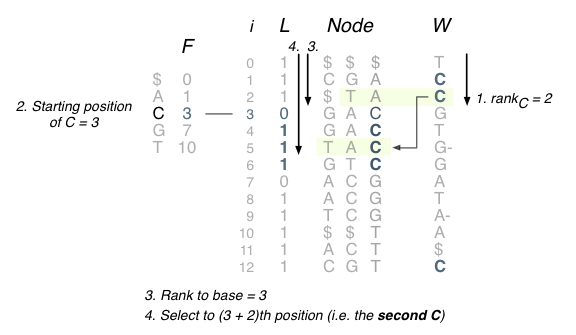
\includegraphics[scale=0.4]{img/fwd.png}
\end{figure}
\end{frame}

\begin{frame}
\frametitle{Backward}
Again thanks to \textbf{Claim 2} following an edge backwardly is equivalent to the corresponding relatively positioned edge. \\
\underline{Example}: \textbf{backward(5)}
\begin{figure}
	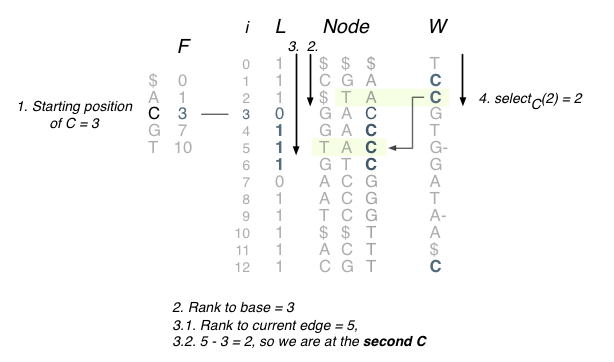
\includegraphics[scale=0.4]{img/bwd.png}
\end{figure}
\end{frame}

\begin{frame}
\frametitle{Supported operations}
At this point we can use \textbf{forward(i)} and \textbf{backward(i)} to support the following operations:
\begin{itemize}
	\item \textbf{outdegree(v)}: \#outgoing edges for node v.\\ $\mathcal{O}$(1) time
	\item \textbf{outgoing(v, c)}: node reached from v through edge labelled c.\\ $\mathcal{O}$(1) time
	\item \textbf{indegree(v)}: \#incoming edges for node v.\\ $\mathcal{O}$(1) time
	\item \textbf{incoming(v, c)}:  predecessor node starting with symbol c, that has an edge to node v.\\ $\mathcal{O}$(k $log\ \sigma$) time
	\item \textbf{label(v)}: complete label of the node v.\\ $\mathcal{O}$(k) time
\end{itemize}
%Note that the parameters to fwd and bwd are index of edges while paramenters for the other operations are node indexes so that we must first select them
\end{frame}

\begin{frame}
\frametitle{Implementing outgoing(v, c)}
Similar to \textbf{forward(i)} but now we want to move starting from a given node v.
\\ \medskip
\underline{Example}: \textbf{outgoing(6, T)}
\begin{figure}
	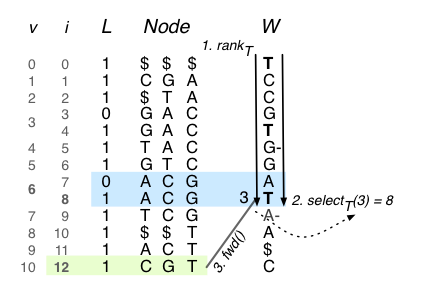
\includegraphics[scale=0.4]{img/outgoing.png}
\end{figure}

\end{frame}

\begin{frame}
\frametitle{Implementing label(v)}
During a traversal we may want to print the node labels out.
\\
We use the position of our node (\textbf{found using select(v)}) as a reverse lookup into \textbf{F} and then we do a series of k backward calls.
\\ \medskip
\underline{Example}: \textbf{label(6)} 
note that in step 1 we do a select(6+1)!
  \begin{columns}
	\column{0.5\textwidth}
	  \begin{figure}
	  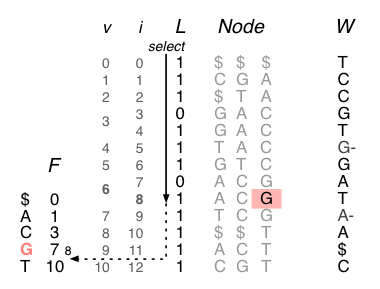
\includegraphics[scale=0.4]{img/label1.png}
	  \end{figure}
	\column{0.5\textwidth}
      \begin{figure}
	   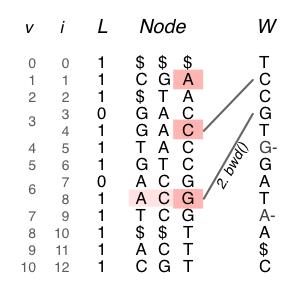
\includegraphics[scale=0.4]{img/label2.png}
      \end{figure}
  \end{columns}
\end{frame}

\begin{frame}
\frametitle{Summarizing the results}
\begin{itemize}
	\item $ m*(2+log\ \sigma +o(1))$ bits, \textcolor{red}{$4m\ +\ o(m)$ bits for DNA}
	\item The size does not depend on k-mer length, so it is effective for large k too.
	\item useful navigation queries are perfomed in constant and in logarithmic time.
\end{itemize}
\end{frame}
 % BOSS   representation for dBGs
% Section 4
\section{Extending BOSS: voBOSS and rBOSS}

\begin{frame}
\begin{center}
\textbf{Where can we go from here?}	
\end{center}

\end{frame}


\begin{frame}
\frametitle{We cannot know the best choice of k a priori}
As seen before construction and navigation of the graph was a space and time bottleneck when acting naively. \\
But we saw how to solve it using compression techniques
\\ \medskip 
Another problem emerges from the fact that state-of-the-art assemblers need to build the de Bruijn graph for multiple values
of K to obtain better sequencing results
\end{frame}


\begin{frame}
\frametitle{The need of the the right k}
\begin{columns}
	\column{0.5\textwidth}
	
	\textbf{Lower k}
	\begin{itemize}
		\item More connections
		\item Less chance of resolving small repeats
		\item Higher k-mer coverage
    \end{itemize}
	\textbf{Higher k}
	\begin{itemize}
		\item Less connections
		\item resolve small repeats
		\item Lower k-mer coverage
	\end{itemize}
	\column{0.5\textwidth}
	\begin{figure}	
		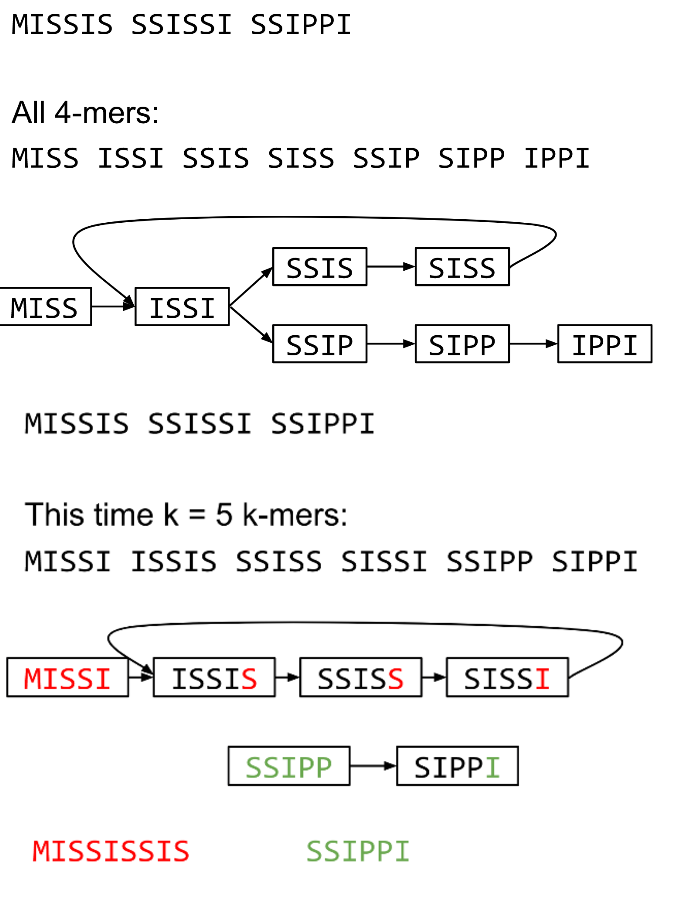
\includegraphics[height=1\textwidth,width=0.8\textwidth]{img/merged-dbg.png}
	\end{figure}
\end{columns}
\end{frame}


\begin{frame}
\frametitle{Variable order dBG (Gagie et al., 2014)}
In 2014 Gagie et al. showed how to augment a succinct de Bruijn graph
representation letting us change order on the fly.
% effectively representing all de Bruijn graphs of order up to some maximum K in a single data structure.
\\ \medskip
Just following a simple observation: deleting the first column of the BOSS-matrix the result is almost the BOSS matrix for a 2nd-order de Bruijn graph.
\\ \medskip
This truncated form of a higher order BOSS differs from the BOSS of a lower order in that some rows are repeated
\\ \medskip
This fact could prevent the BOSS representation from working properly. 
\end{frame}

\begin{frame}
\frametitle{Fixing it}
Instead of trying to apply forward, backward and
lastchar directly to nodes in the lower-order-graphs, we augment the BOSS representation of
the original graph to support the following three queries:
\begin{itemize}
	\item \textbf{shorter(v, k)} returns the node whose label is the last k characters of v’s label;
	\item \textbf{longer(v, k)} lists nodes whose labels have length k ≤ K and end with v’s label;
	\item \textbf{maxlen(v, a)} returns some node in the original graph whose label ends with v’s. label, and that has an outgoing edge labelled a, or NULL otherwise.
\end{itemize}
\end{frame}


\begin{frame}
\frametitle{}
If v is a node in the original graph then we
can use the BOSS implementations of forward, backward and lastchar.
\\ \medskip
Otherwise, if v’s label has length $k_v \leq k$ then:
\begin{itemize}
	\item \textbf{fwd(v, a) = shorter(fwd(maxlen(v, a), a), $k_v$ )}
	\item \textbf{bwd(v) = shorter(bwd(maxlen(longer(v,$k_v$+ 1), ∗)), $k_v$ )}
	\item \textbf{lastchar(maxlen(v, ∗))}
\end{itemize}
\end{frame}


\begin{frame}
\frametitle{Implementing shorter and longer}
To implement shorter and longer, we store a wavelet tree over the sequence $L^∗$
in which $L^* [i]$ is the length of the longest common suffix of Node[i] and Node[i+1].
\\ \medskip
This takes $\mathcal{O}(log\ K)$ bits per (K + 1)-tuple in the matrix.\\
To save space, we can omit Ks in $L^∗$, since they correspond to 0s in L and indicate that Node[i] and Node[i+1] are in the interval of the same node in the original graph;
\\ \medskip 
the wavelet tree then takes $\mathcal{O}(log\ K)$ bits per node in the original graph and $\mathcal{O}(n\ log\ K)$  bits in total.
\\ \medskip
In our example, $L^∗ = [0, 1, 0, 3, 2, 1, 0, 3, 2, 0, 1, 1 ]$
(we can omit the 3s to save space).
\end{frame}


\begin{frame}
\frametitle{Conclusions: Versatility of BOSS}
The goodness of the BOSS representation was highlighted both by the original results and by all the extensions that came out in the following years.
\\ \medskip
Infact we just saw how to use BOSS to deal with variable order de Bruijn graphs.
\\ \medskip
But the improvements are not over ...
\end{frame}


\begin{frame}
\frametitle{Concluding: simulating the overlap graph}
In 2019 Dominguez et al [3] showed that BOSS can be extended even more arriving to simulate the overlap graph on the fly
\\ \medskip
The authors observed that overlaps between reads can be computed using voBOSS
\end{frame}

\begin{frame}
\frametitle{Link between variable-order and overlaps}
- extend a unary path using solid nodes as much as possible; 
\\ \medskip
- if a solid node v without outgoing edges is reached, then decrease its order with shorter to retrieve the nodes that represent both a suffix of v and a prefix of some other read.
\\ \medskip
- from these nodes, retrieve the overlapping solid nodes of v by using forward and continue the graph right traversal from one of them.
\end{frame}

\begin{frame}
\frametitle{When does shorter work correctly?}
Since shorter does not ensure that the label of the output node appears as a prefix in the set of reads we need some precise conditions:
\begin{lemma}
	In voBOSS, applying the operation shorter to a node v of order $k' \leq k$ will
	return a node u of order $k'' < k'$ that encodes a forward overlap for v \\
	$\Leftrightarrow$\\
	u[1] is a linker node contained by v.
\end{lemma}
\end{frame}

\begin{frame}
\frametitle{rBOSS fundamentals}
We are ready to define the two operations needed to compute overlaps using voBOSS:
\begin{itemize}
	\item \textbf{nextcontained(v)}: returns the greatest linker node v , in lexicographical order, whose llabel represents both a suffix of v and a prefix of some other node in G.
	\item \textbf{buildL(v,m)}: returns the set of all the linker nodes contained by v that represent a suffix of v
	of length $\geq m$.
\end{itemize}
the second operation is needed since a node might have more than one contained linker node, and those linkers whose \textbf{llabel} is of length $\geq m$ represent edges in the overlap graph.
\end{frame}

\begin{frame}
\frametitle{Final remarks}
\begin{itemize}
	\item if we chose $k = z + 1$ to build voBOSS we are simulating the full overlap graph in compressed space.\\
	The edges are not stored explicitly, but computed on the
	fly by first obtaining L = buildL(v, m), and then following the dBG outgoing edges of every l ∈ L.
	\item This extension substitutes the \textbf{LCS} over \textbf{L} with a compacted trie to achieve fast implementation of \textbf{buildL(v,m)}.
	
\end{itemize}

\end{frame}

 % voBOSS representation for dBGs
%%%%%%%%%%%%%%%%%%%%%%%%%%%%%%%%%%%%%%%%%%%%%%%%%%%%%%%%%%%%%%%%%%%%%%%%%%%%%%%%
%%%%%%%%%%%%%%%%%%%%%%%%%% REFERENCES %%%%%%%%%%%%%%%%%%%%%%%%%%%%%%%%%%%%%%%%%
%%%%%%%%%%%%%%%%%%%%%%%%%%%%%%%%%%%%%%%%%%%%%%%%%%%%%%%%%%%%%%%%%%%%%%%%%%%%%%%%

\section{} % or \section*{}
\begin{frame}
\frametitle{References}
\begin{enumerate}
	\item Alexander Bowe, Taku Onodera, Kunihiko Sadakane, and Tetsuo Shibuya. Succinct de Bruijn
	graphs. In Proc. 12th International Workshop on Algorithms in Bioinformatics (WABI), pages
	225–235, 2012.
	\item Christina Boucher, Alexander Bowe, Travis Gagie, Simon J Puglisi, and Kunihiko Sadakane.
	Variable-order de Bruijn graphs. In Proc. 25th Data Compression Conference (DCC), pages
	383–392, 2015.
	\item 	Diego Díaz-Domínguez, Travis Gagie, Gonzalo Navarro. Simulating the DNA String Graph in Succinct Space
\end{enumerate}
\end{frame}

\begin{frame}
Thanks for the attention! \\ \medskip
Any question?
\end{frame}
%%%%%%%%%%%%%%%%%%%%%%%%%%%%%%%%%%%%%%%%%%%%%%%%%%%%%%%%%%%%%%%%%%%%%%%%%%%%%%%%
%%%%%%%%%%%%%%%%%%%%%%%%%%%%%%%%%%%%%%%%%%%%%%%%%%%%%%%%%%%%%%%%%%%%%%%%%%%%%%%%
%%%%%%%%%%%%%%%%%%%%%%%%%%%%%%%%%%%%%%%%%%%%%%%%%%%%%%%%%%%%%%%%%%%%%%%%%%%%%%%%
\end{document}
